% !TEX root = ../foresight.tex

\section{Results}

In this section we provide experimental results that validate our approach. A video accompanies this submission and is available at \ja{add link to website}.

\subsection{Localization Accuracy}

We tested our localization framework by emulating the car's ultra-wideband
sensor configuration inside a motion capture system. We placed motion capture
markers on the quadrotor and on each ultra-wideband sensor. This allowed us to
obtain the absolute position of the quadrotor and UWBs in the same coordinate
frame. We then flew the quadrotor inside the motion capture system and recorded
its predicted position determined by our localization and absolute position
using the motion capture markers. The average error in our localization was
13.7 cm, or 35.9\% the length of the quadrotor. Fig.~\ref{fig:localization}
shows how our localization compares to the ground truth. The green and red
lines respectively show the ground truth and predicted positions of the
quadrotor.\ja{How come it is worse than the reported errors in the UWB paper that we are citing?}

\begin{figure}

    \centering

    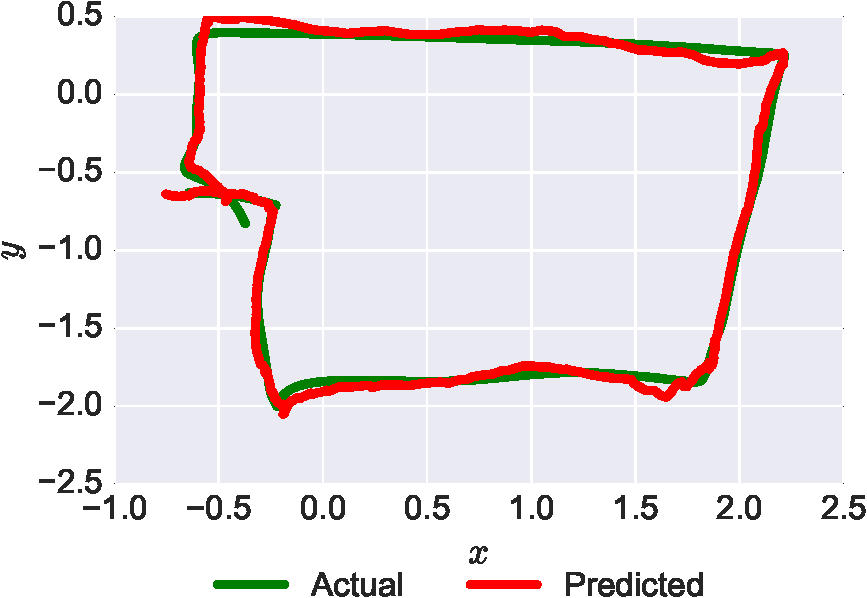
\includegraphics[width=0.7\linewidth]{localization}

    \caption{Comparison of our localization method with respect to
    ground truth. Ground truth was supplied by a motion capture system.}

    \label{fig:localization}

\end{figure}

\subsection{Experimental Setup}

For our experiments, we used a Toyota Prius with a SICK LMS1xx mounted on the
front of the car and six Decawave TREK1000 ultra-wideband radios mounted on the
roof and front bumper of the car. A platform for the quadrotor to take off and
land is attached to the front bumper of the Prius. We used a Parrot Bebop 2
quadrotor with a Decawave TREK1000 mounted on the battery.  Fig.~\ref{fig:car}
and Fig.~\ref{fig:bebop-actual} show the Toyota Prius and modified Bebop 2
quadrotor used in the experiments.

\begin{figure}[h!]

    \centering

    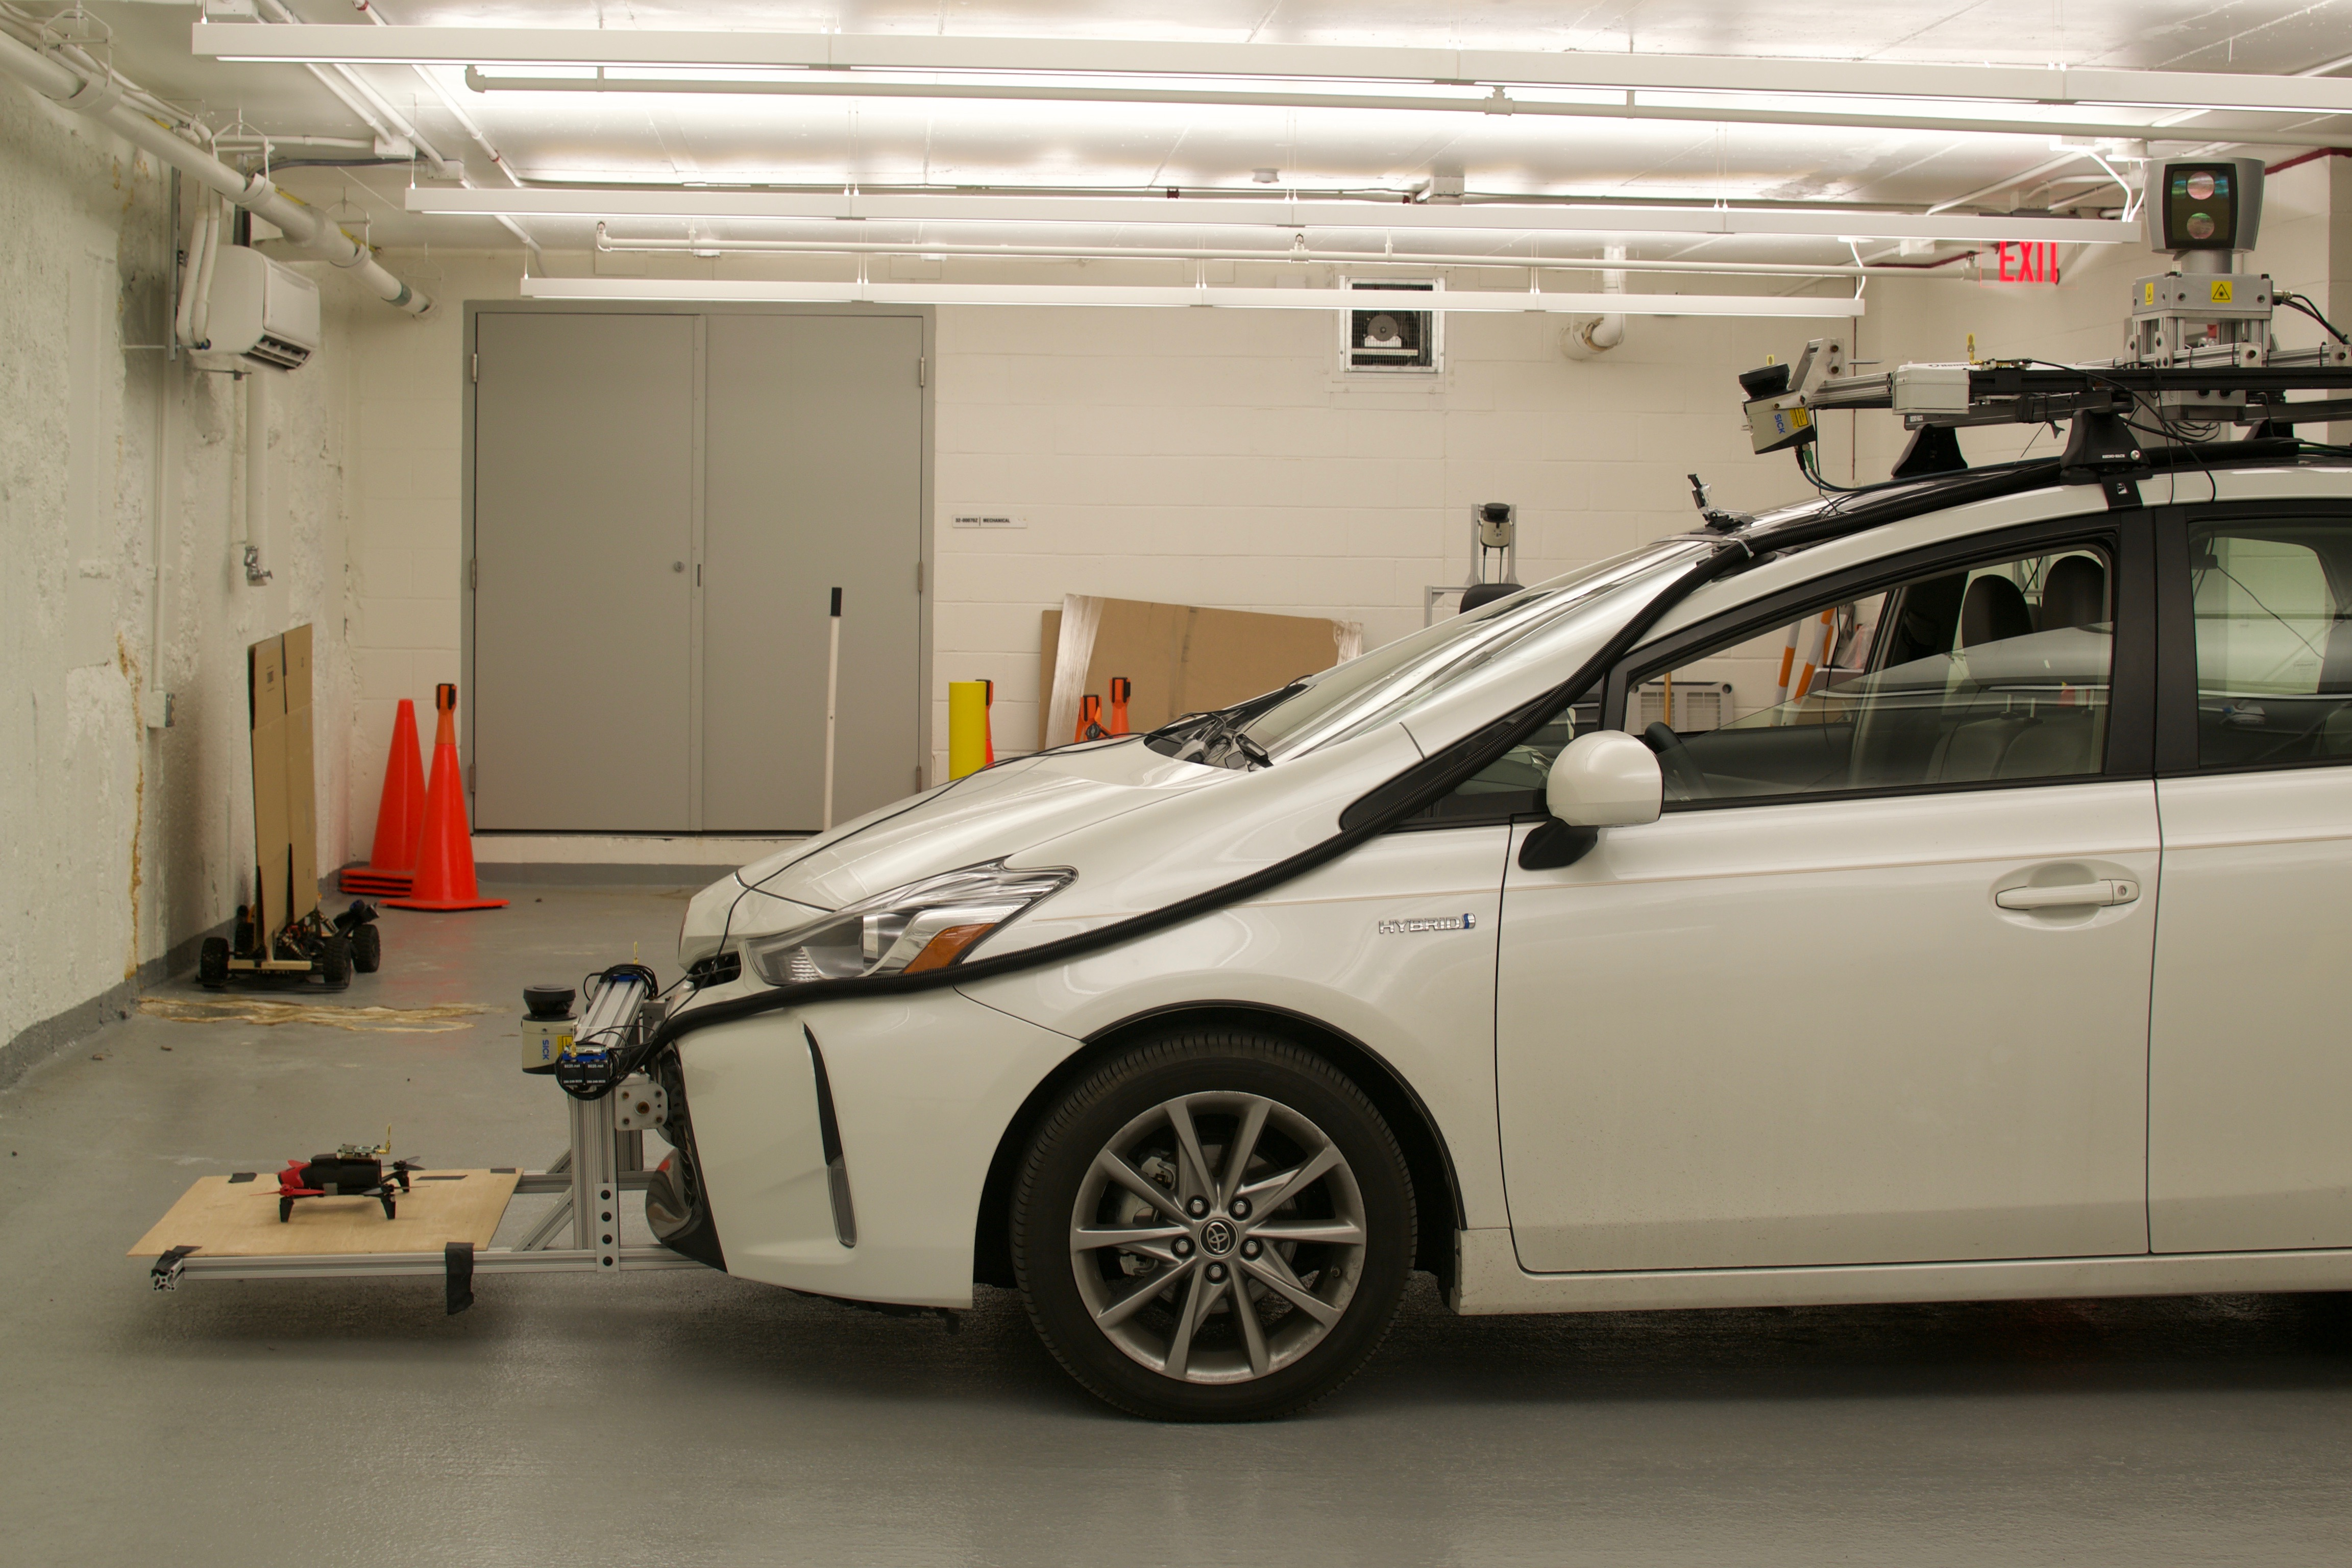
\includegraphics[width=0.49\linewidth]{car-side-view}
    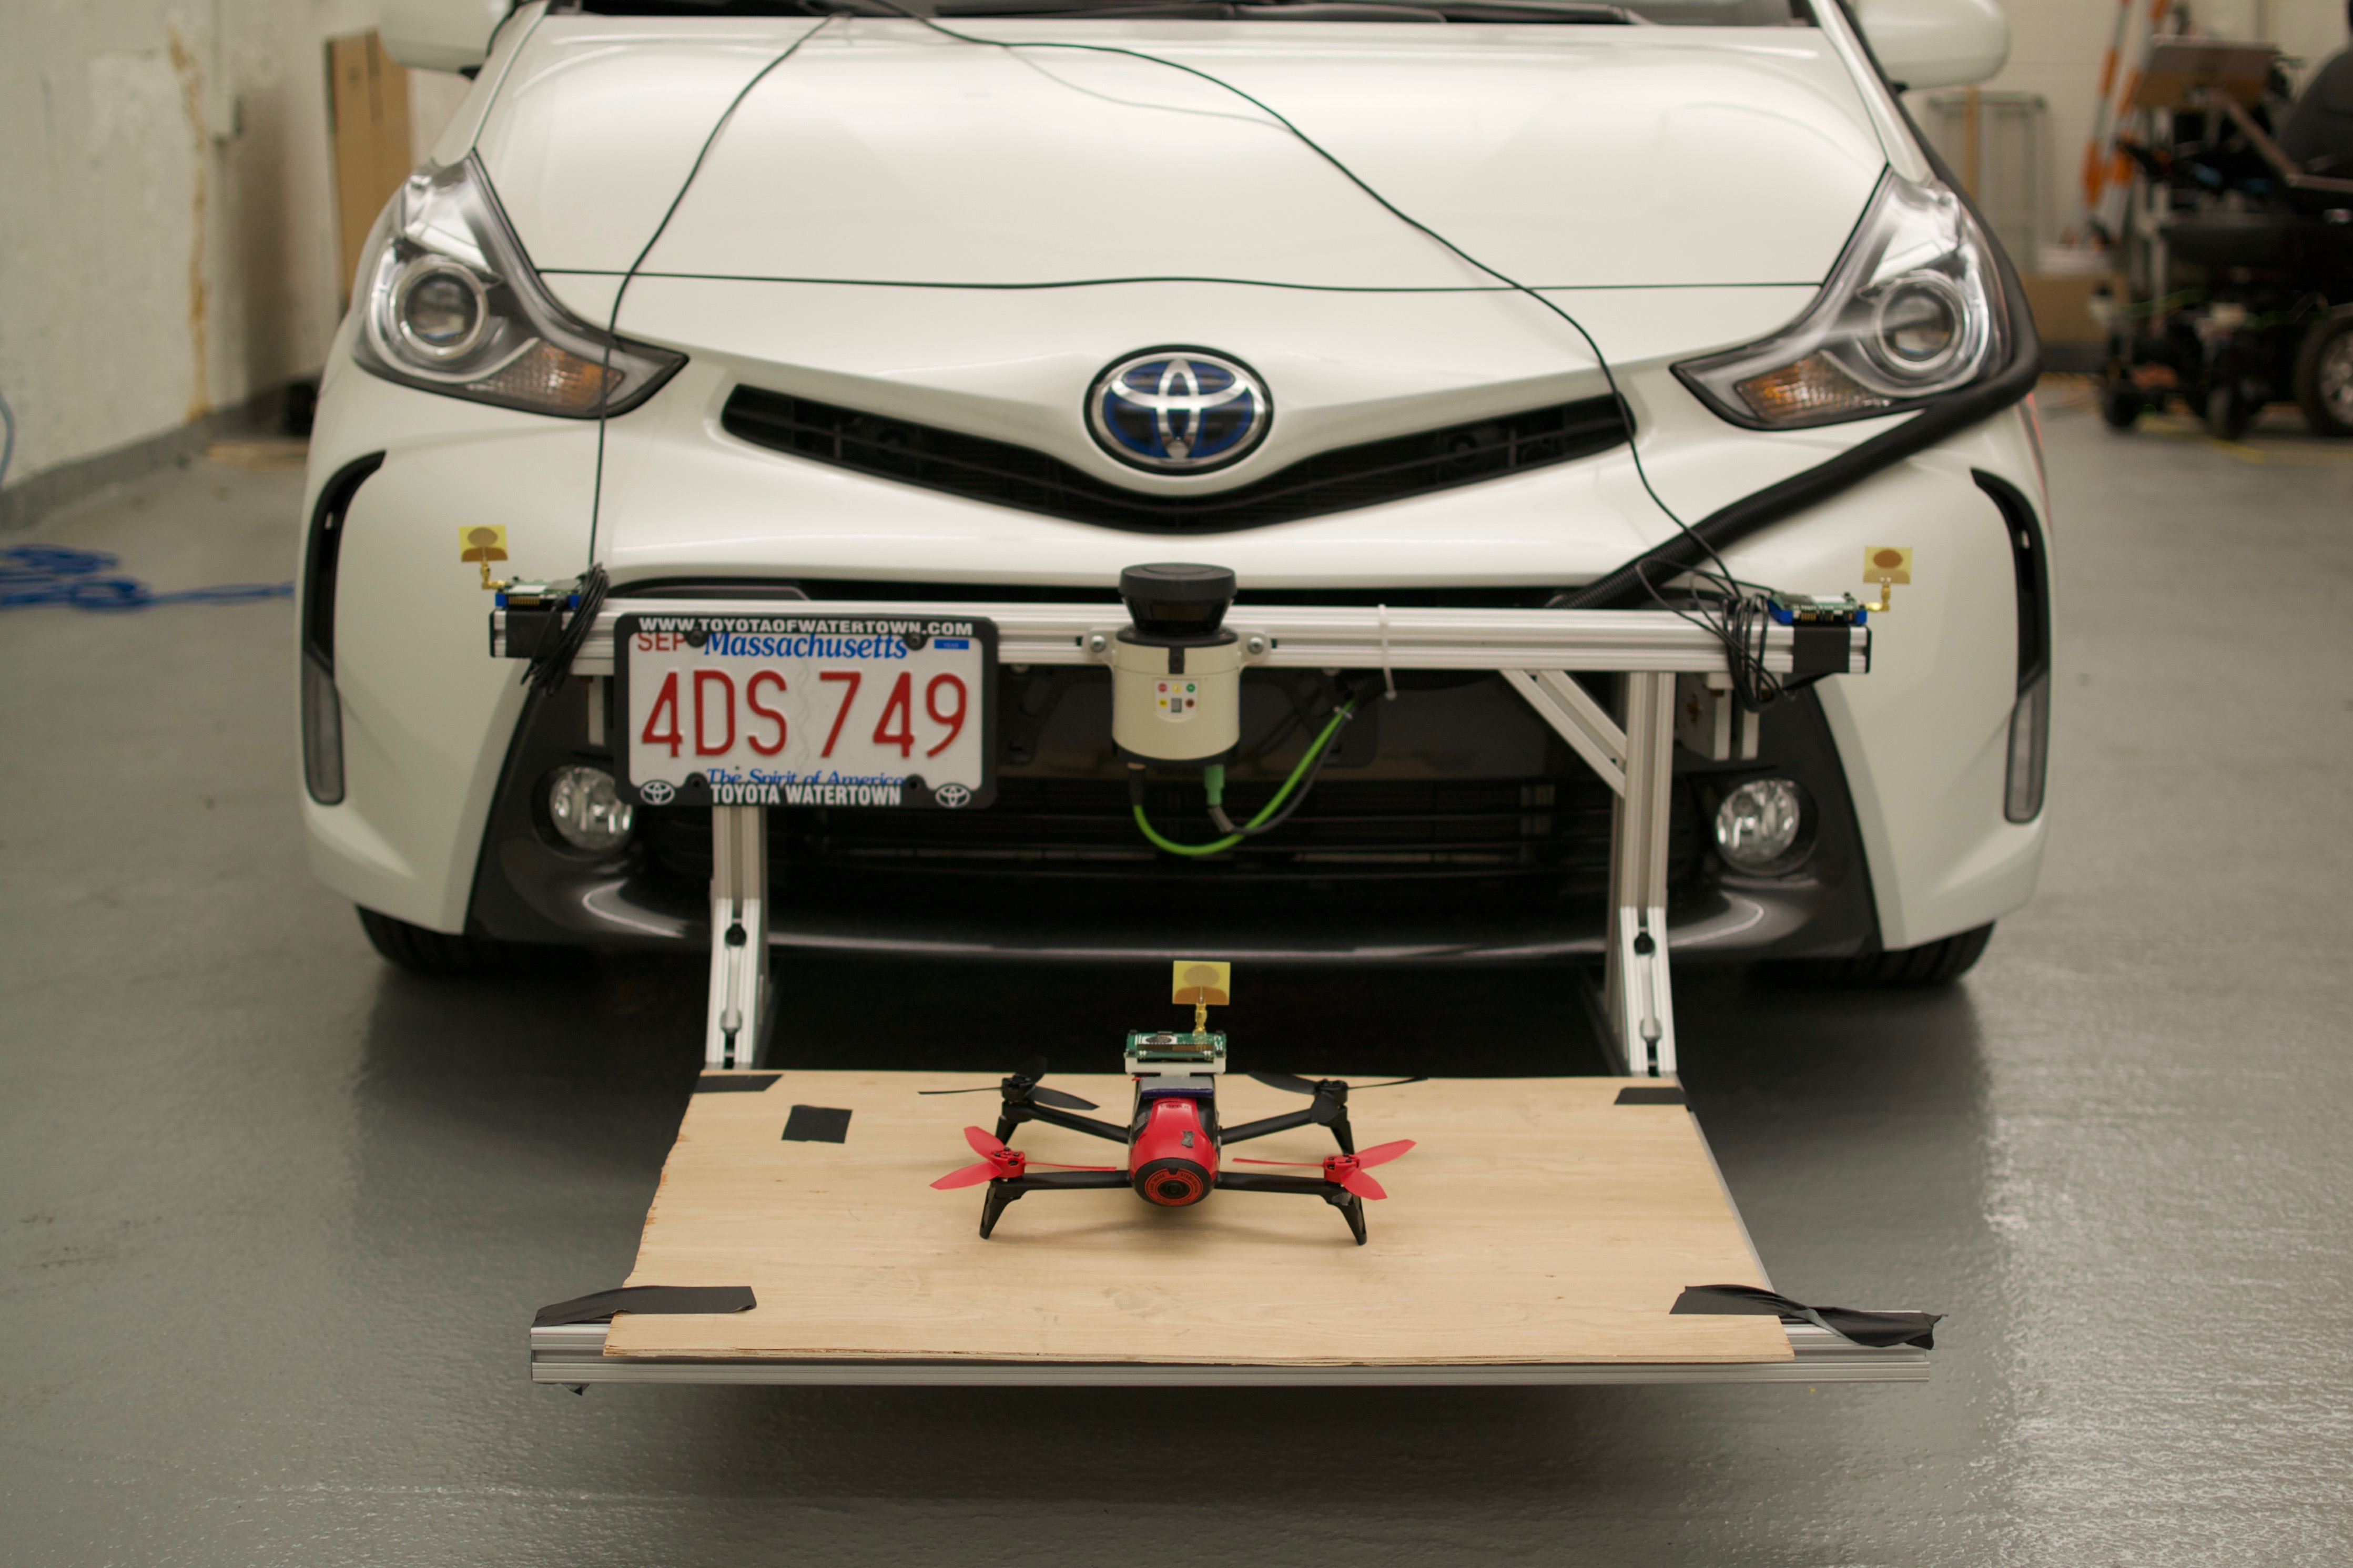
\includegraphics[width=0.49\linewidth]{car-close-up}

    \caption{}

    \label{fig:car}

\end{figure}

% \begin{figure}[h!]
%
%     \centering
%
%     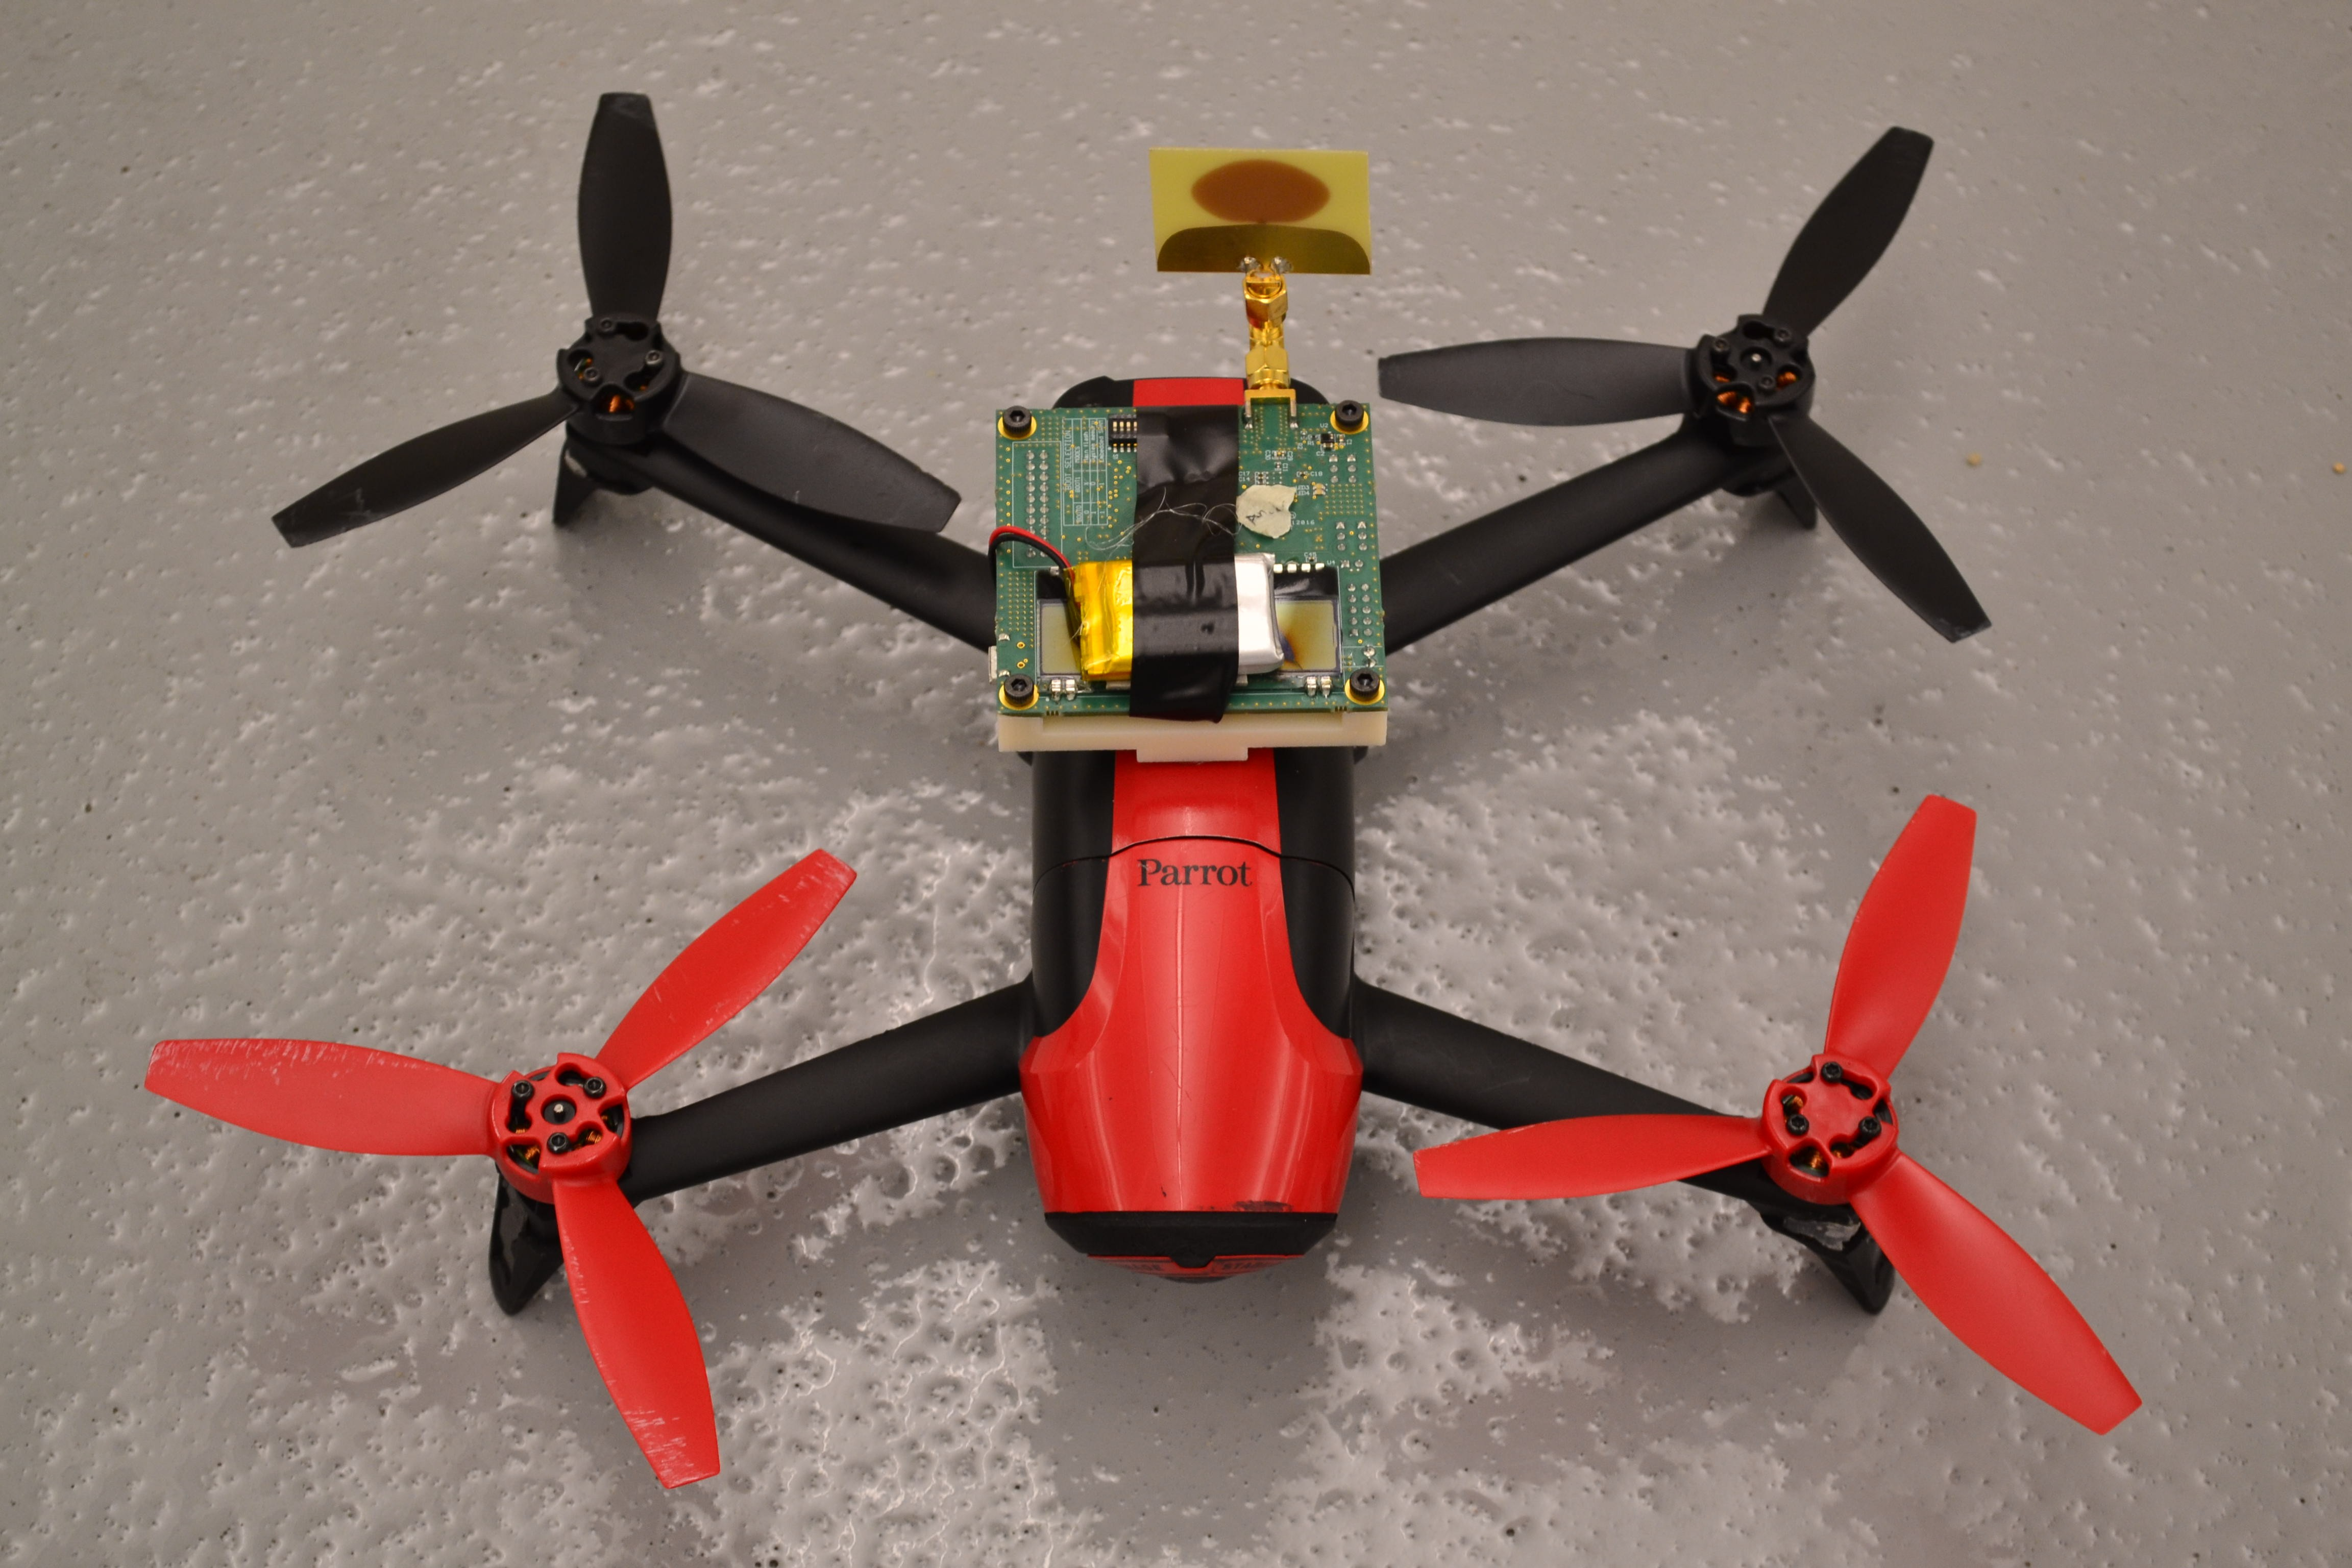
\includegraphics[width=0.7\linewidth]{bebop-actual}
%     % 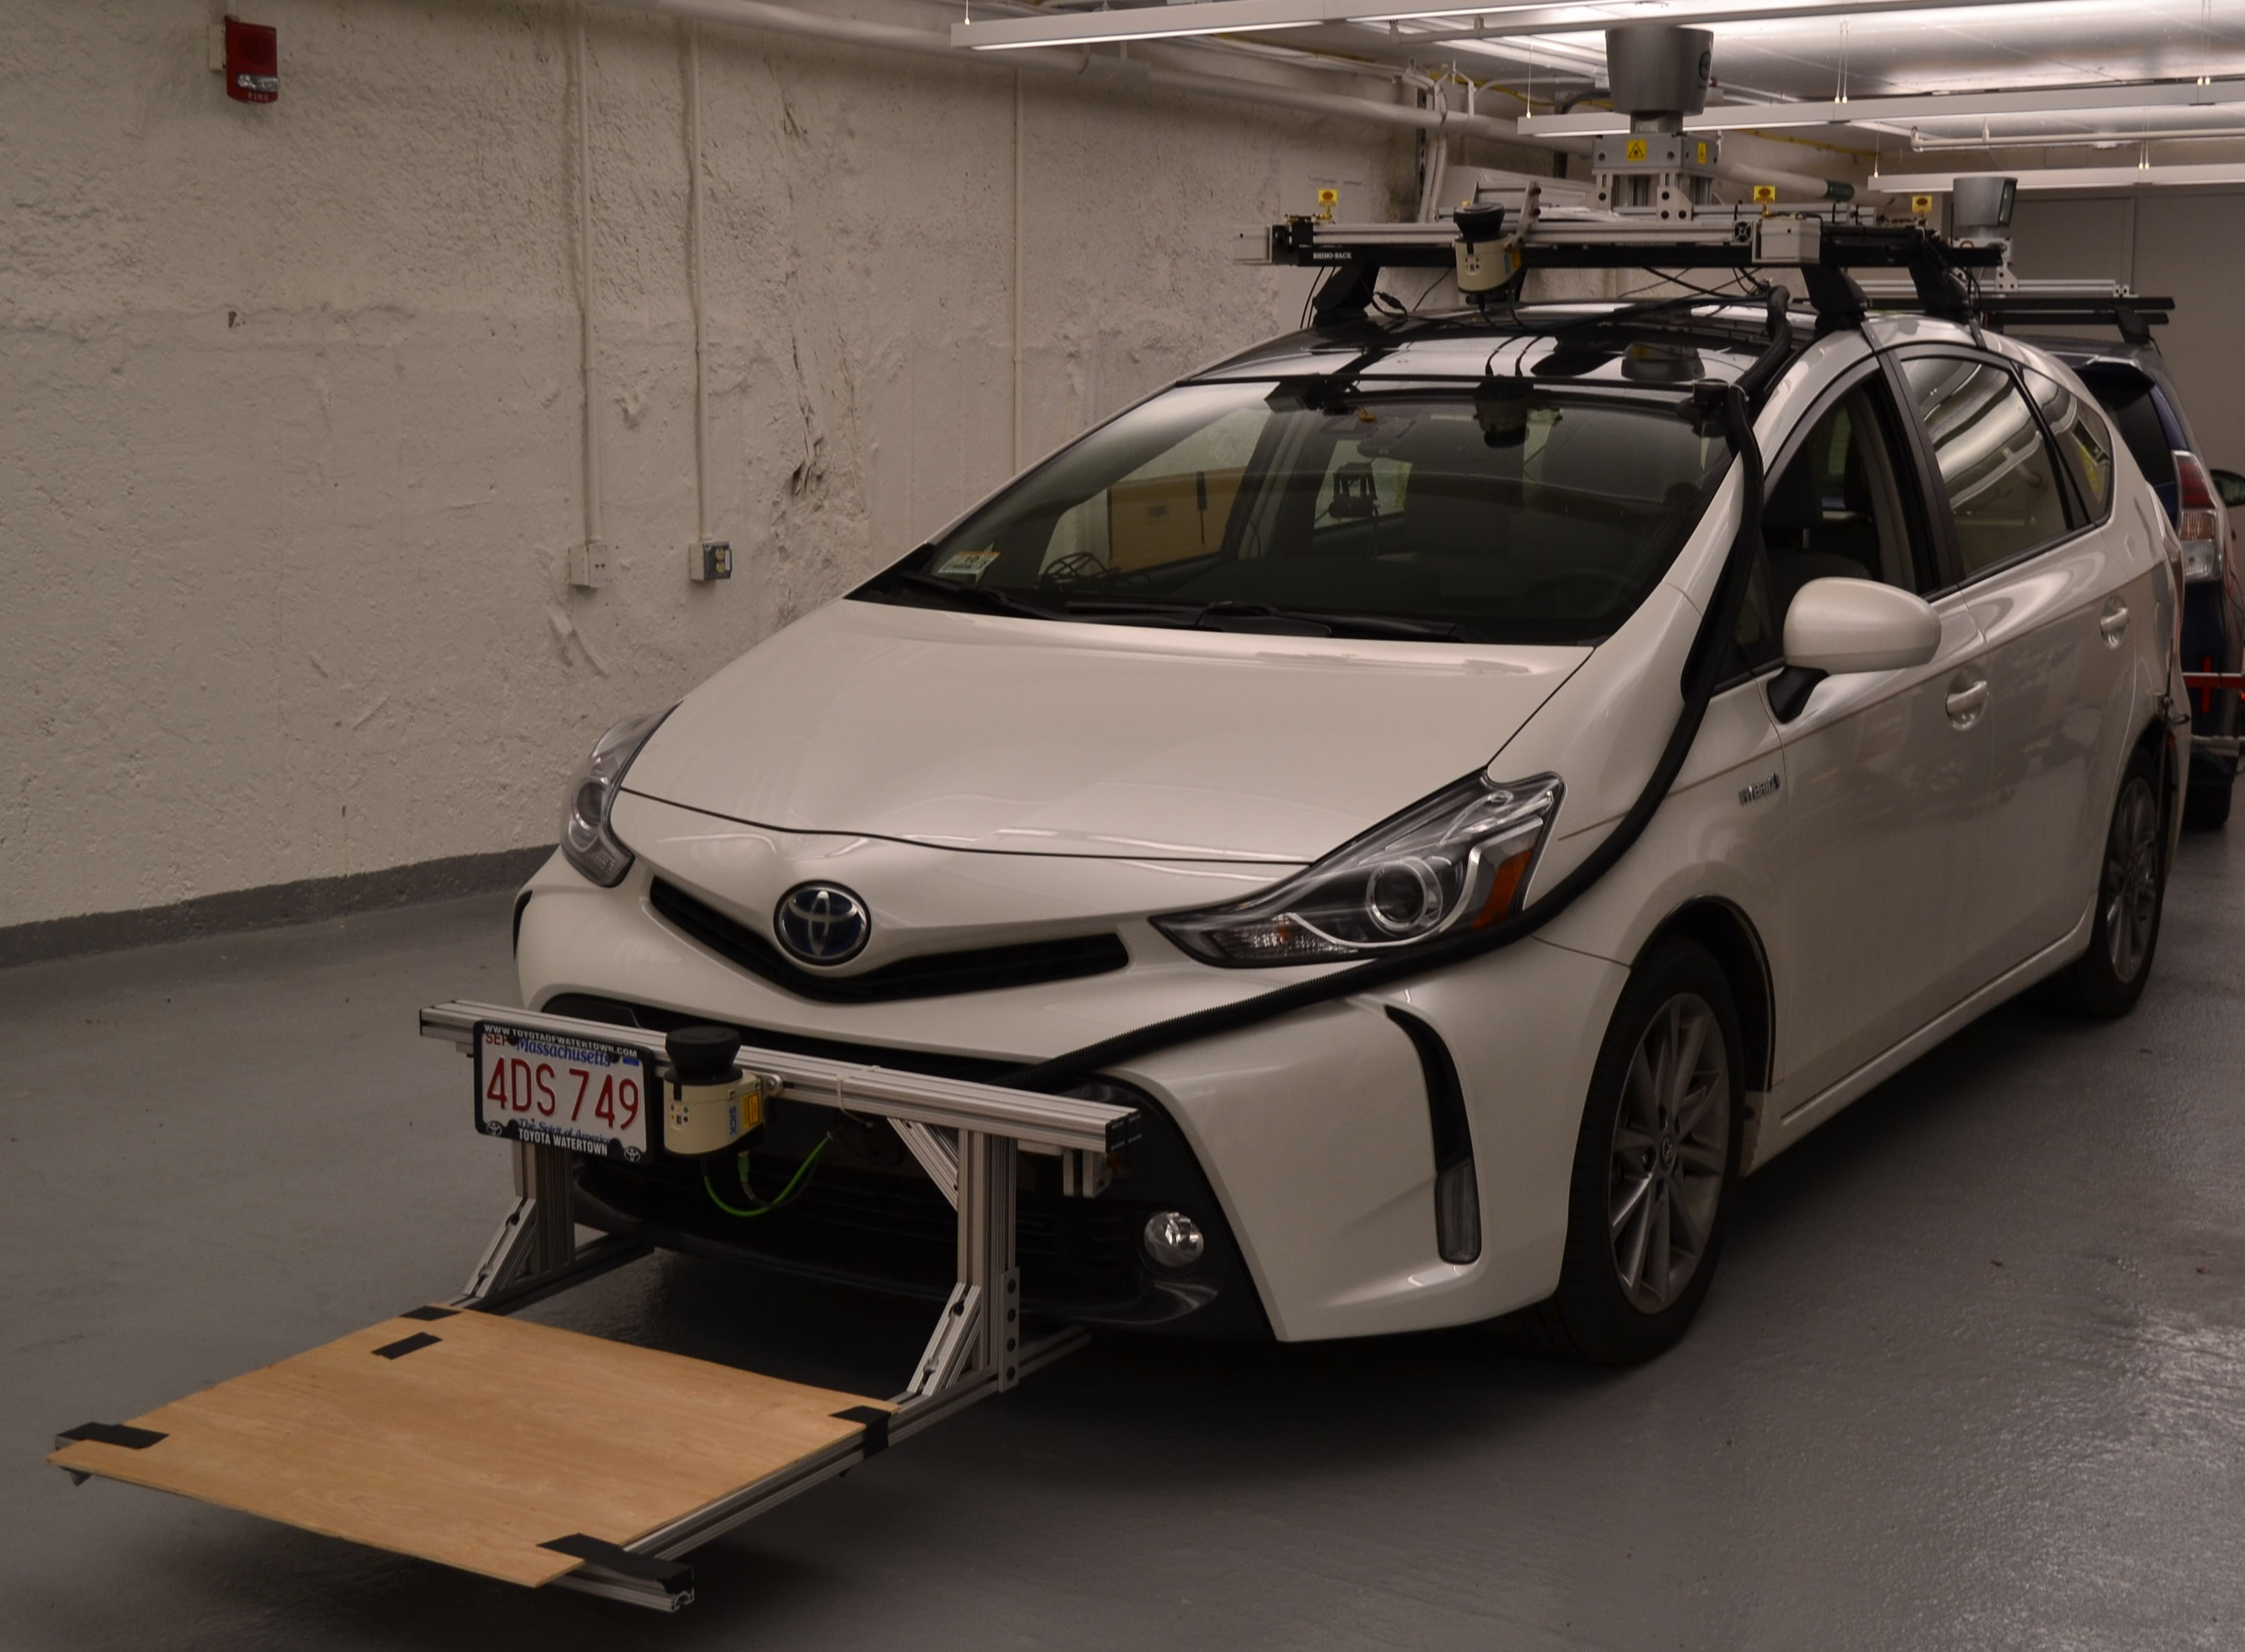
\includegraphics[height=3.8cm]{car}
%     % 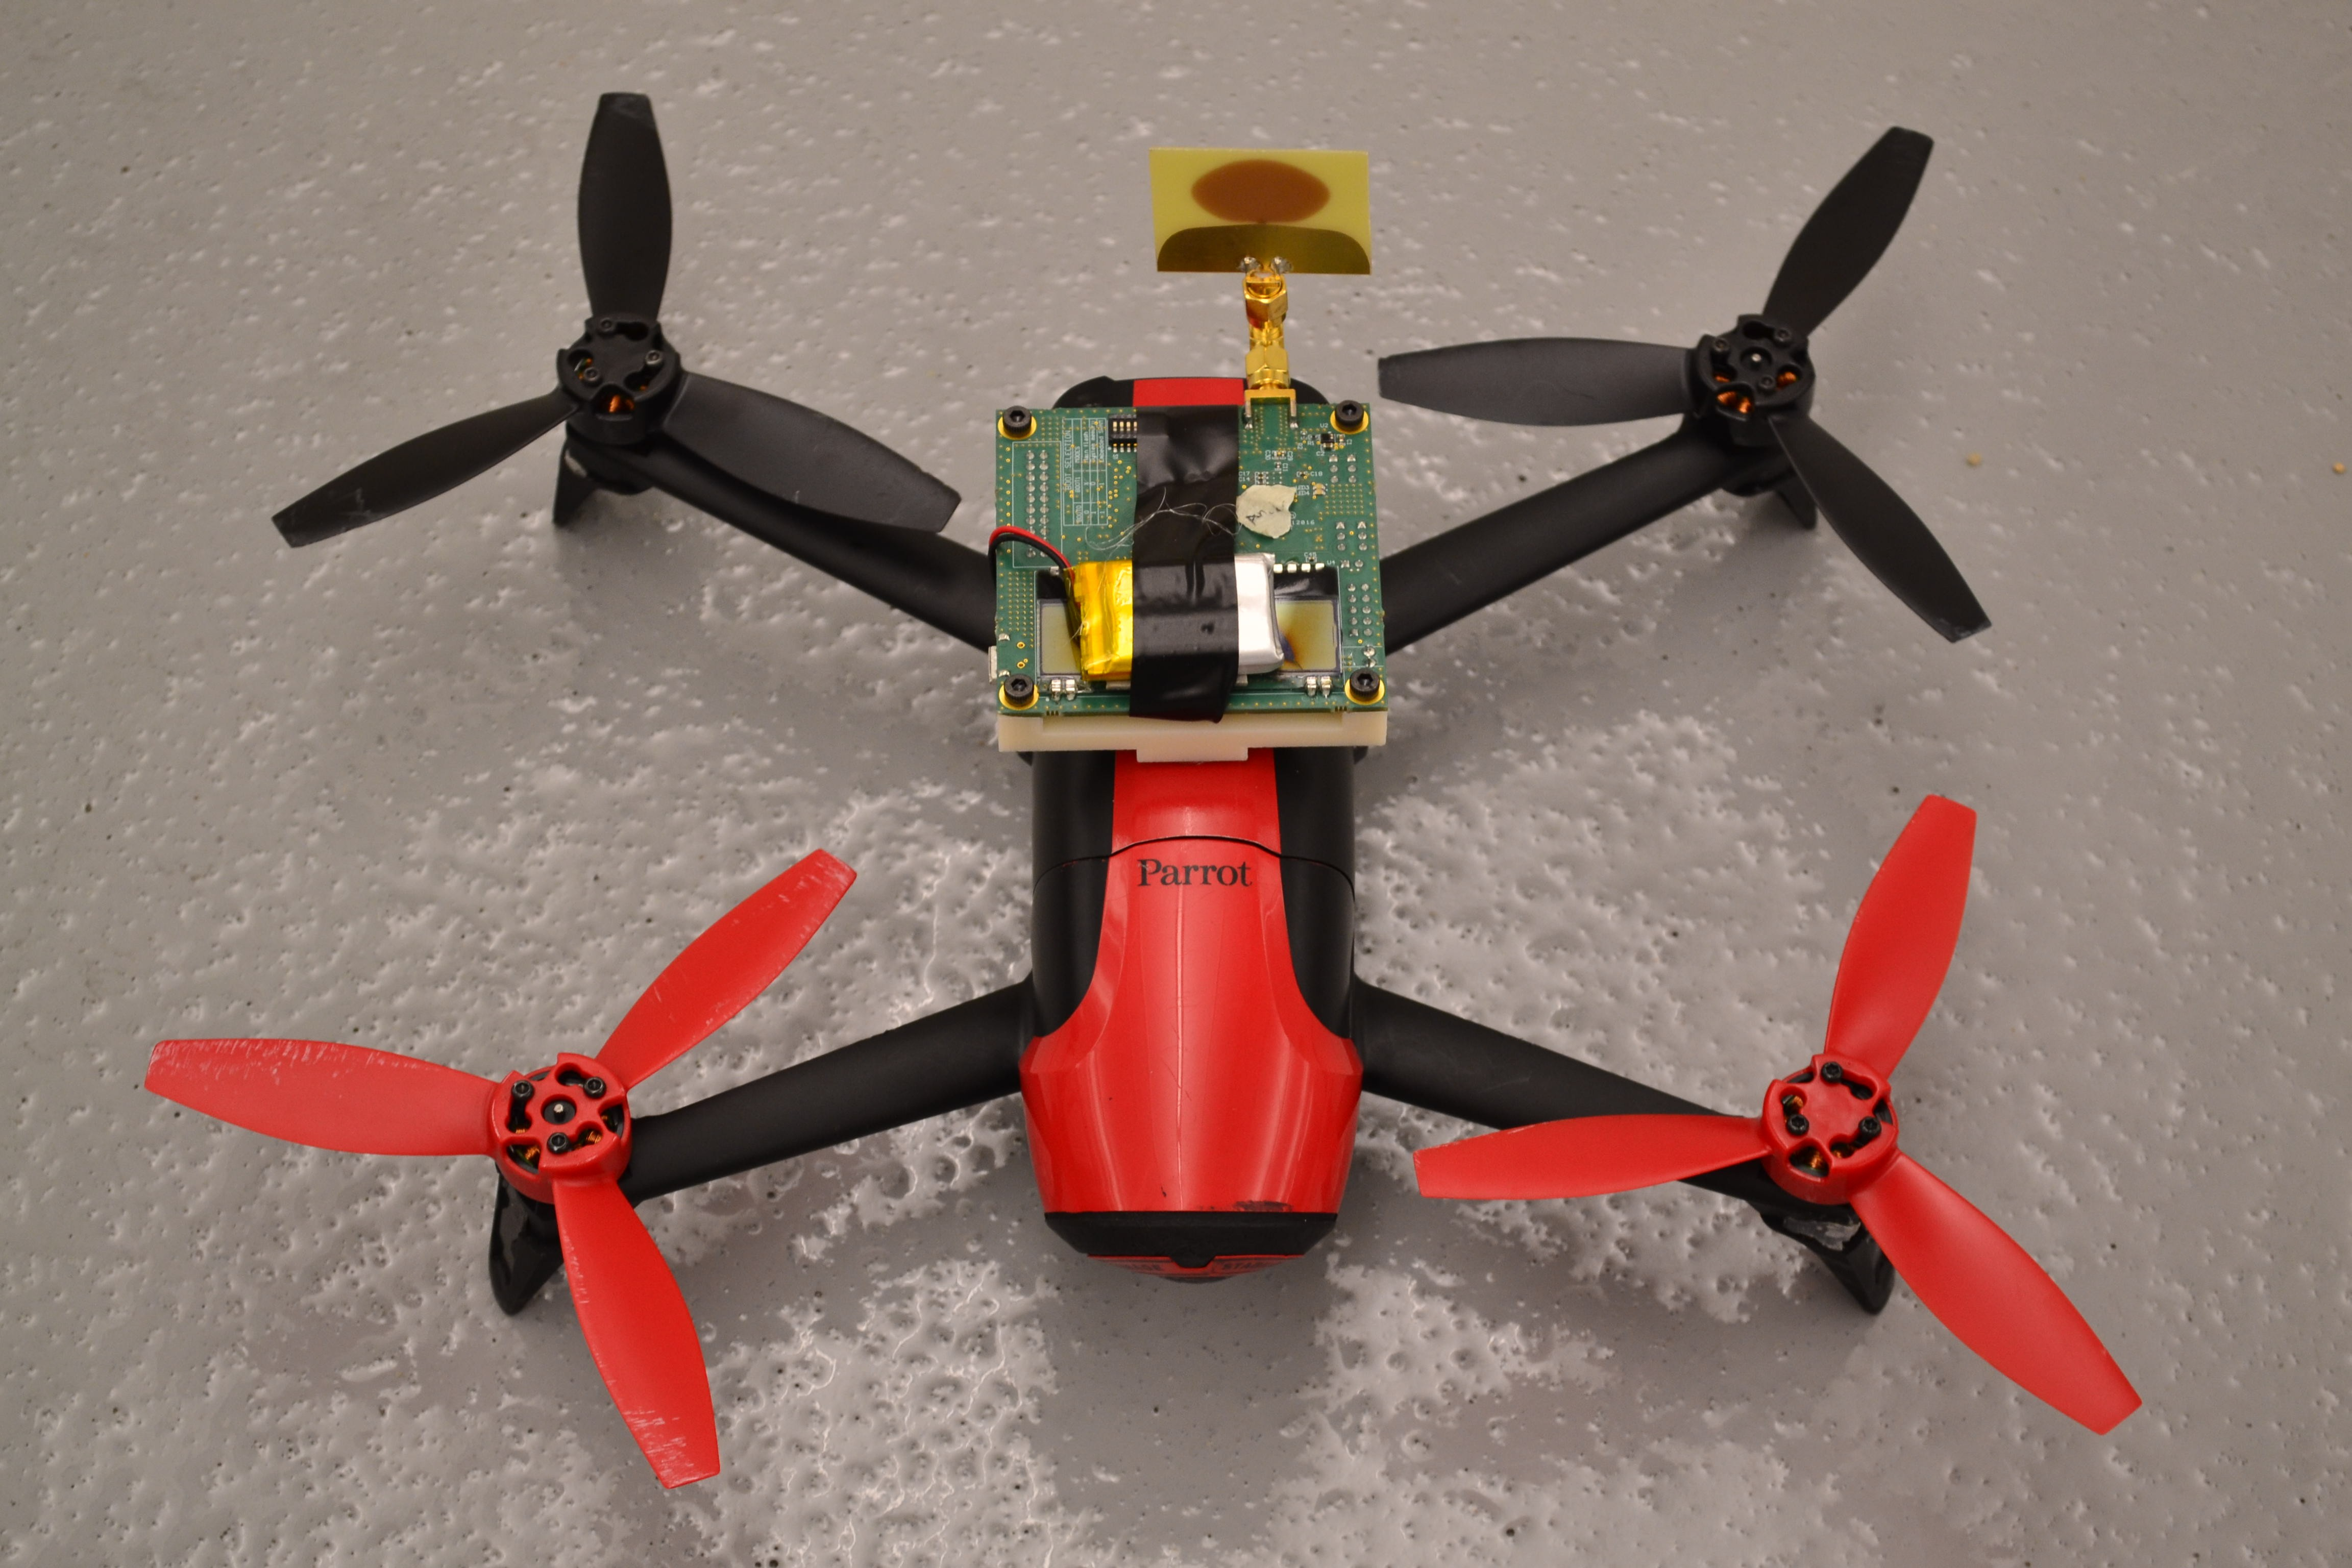
\includegraphics[height=3.8cm]{bebop-actual}
%
%     \caption{}
%
%     \label{fig:bebop-actual}
%
% \end{figure}

Our experimental scenario involves a car preparing to leave a garage with a
significant blind spot. The car is unable to sense around the corner to
determine if there are pedestrians or other cars that may obstruct its path.
Our quadrotor takes off from the car's front bumper platform and autonomously
flies out of the garage and looks around the corner. The car is then able to
leave the garage when there are no more pedestrians detected by the quadrotor.
Once the car is ready to return, it backs up into the garage. The quadrotor
then follows the car into the garage and autonomously lands on the platform.

\subsection{Experiment With Quadrotor}

\subsubsection{Looking Around the Corner}

Fig.~\ref{fig:experiment} shows snapshots of the experiment as it progressed.
The first column is a third person angle of the Prius and the quadrotor. The
second column shows frames from the quadrotor's on-board camera along with
object detection and classifications from the convolutional neural net. The
third column is a visualization of the sensor data from the car, the bounding
polygon, blind regions, and the quadrotor's plan. Each row shows a single
snapshot from the experiment.

We can see from the snapshots that the quadrotor is able to successfully take
off from the car, use the laser scan to find the blind regions, and plan a path
to look around the corner in the garage. From the last row, we also see that
our system is able to detect that there is a pedestrian around the corner and
provide the bounding box to the either the driver or an autonomous system
operating the car.

Note that even though the quadrotor is not equipped with the sensors needed to
perform robust 3D obstacle avoidance, it is able to avoid collisions and fly
through the open garage door using the laser scan from the car.

\begin{figure}[h!]

    \centering

    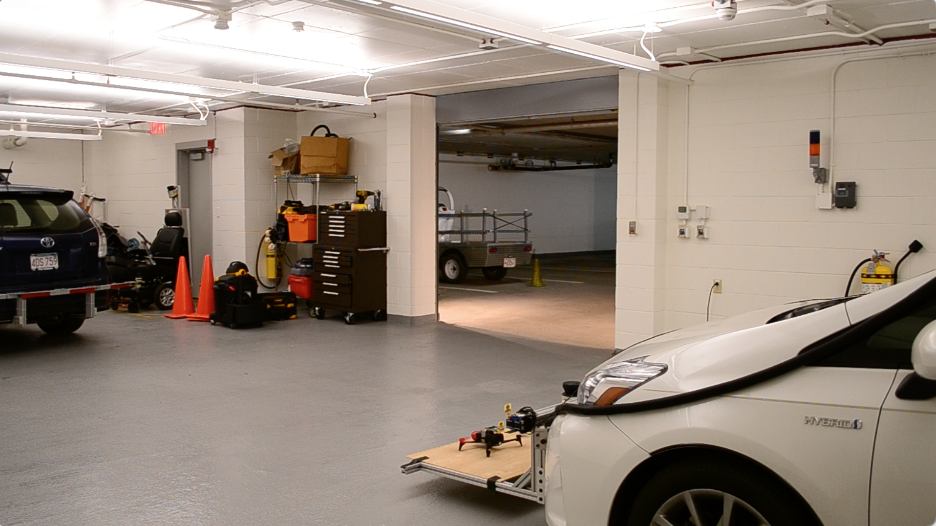
\includegraphics[width=0.35\linewidth]{00-third-person}
    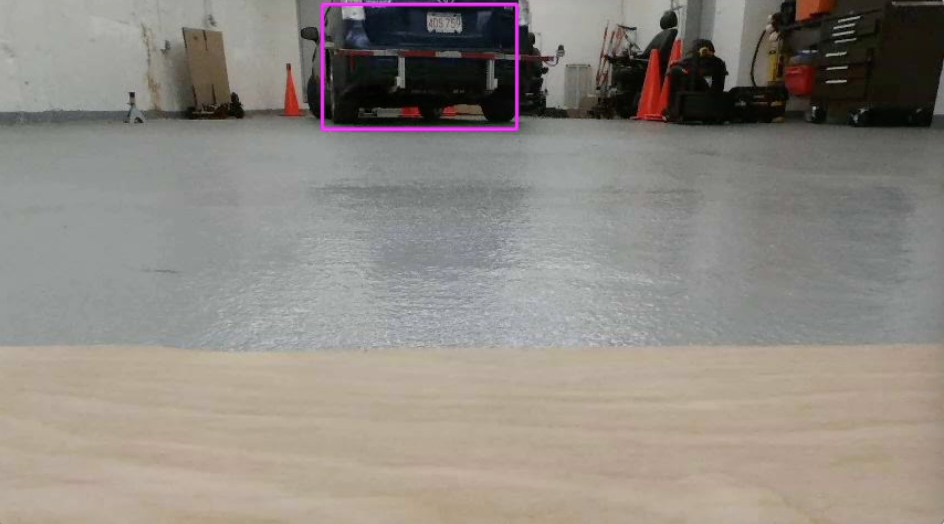
\includegraphics[width=0.35\linewidth]{00-quad-cam}
    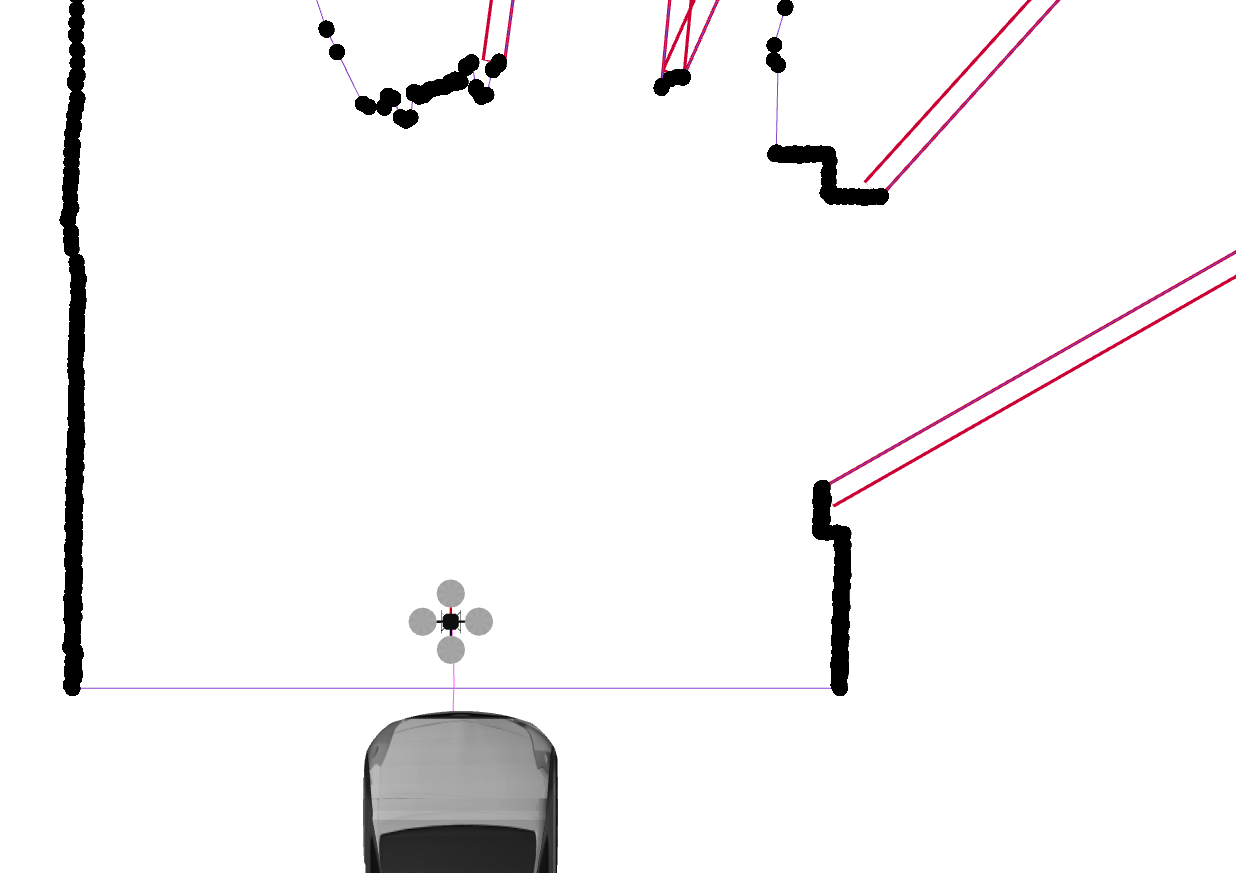
\includegraphics[width=0.28\linewidth]{00-planner-step} \\
    \vspace*{1mm}
    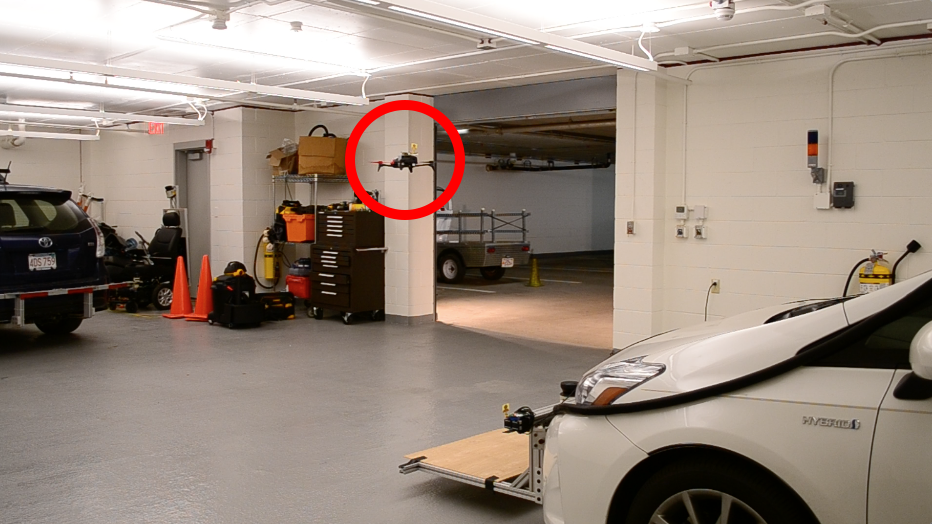
\includegraphics[width=0.35\linewidth]{01-third-person}
    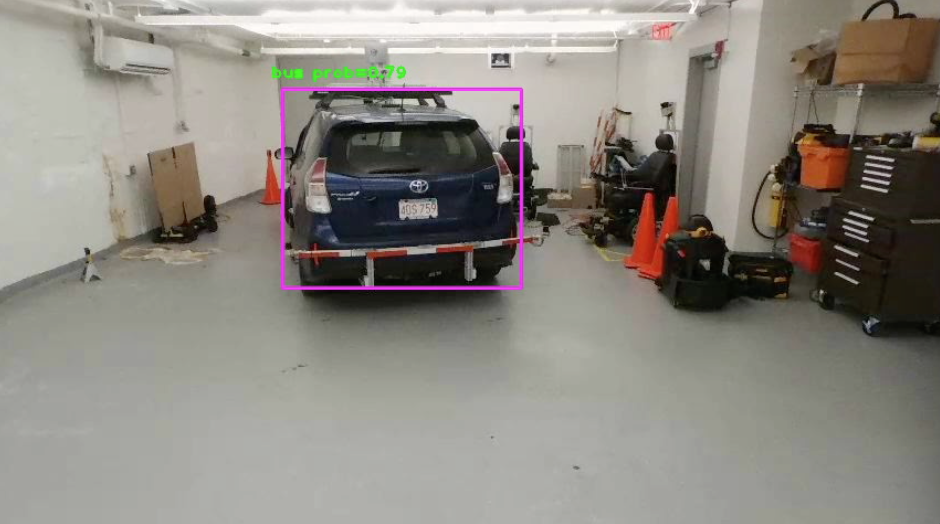
\includegraphics[width=0.35\linewidth]{01-quad-cam}
    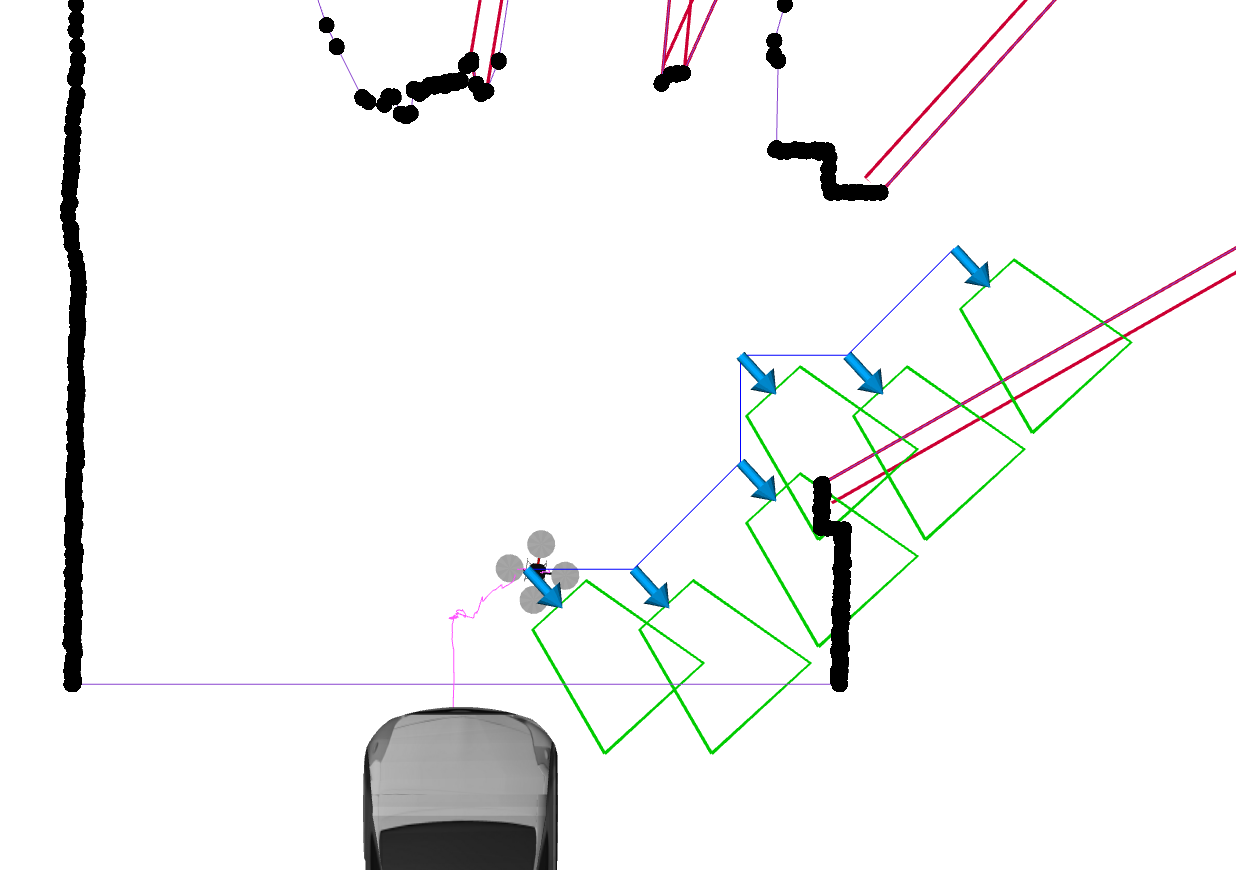
\includegraphics[width=0.28\linewidth]{01-planner-step} \\
    \vspace*{1mm}
    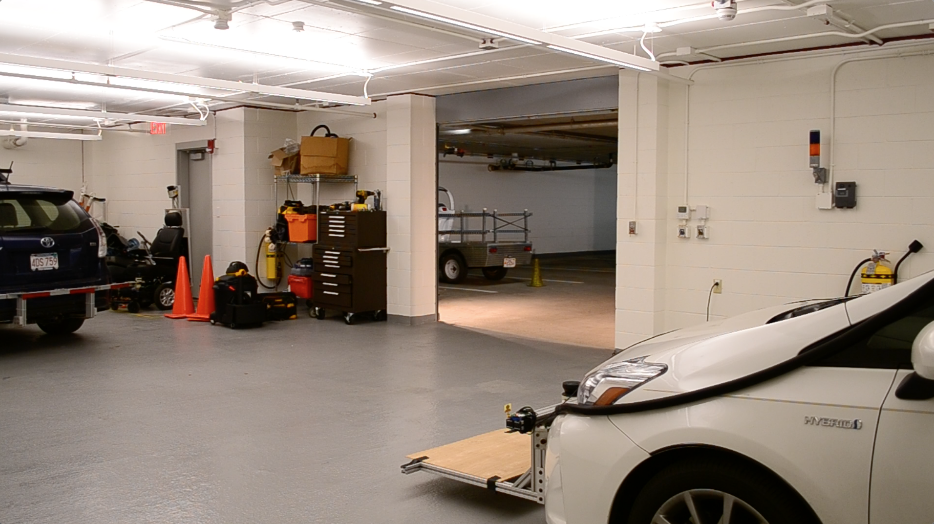
\includegraphics[width=0.35\linewidth]{02-third-person}
    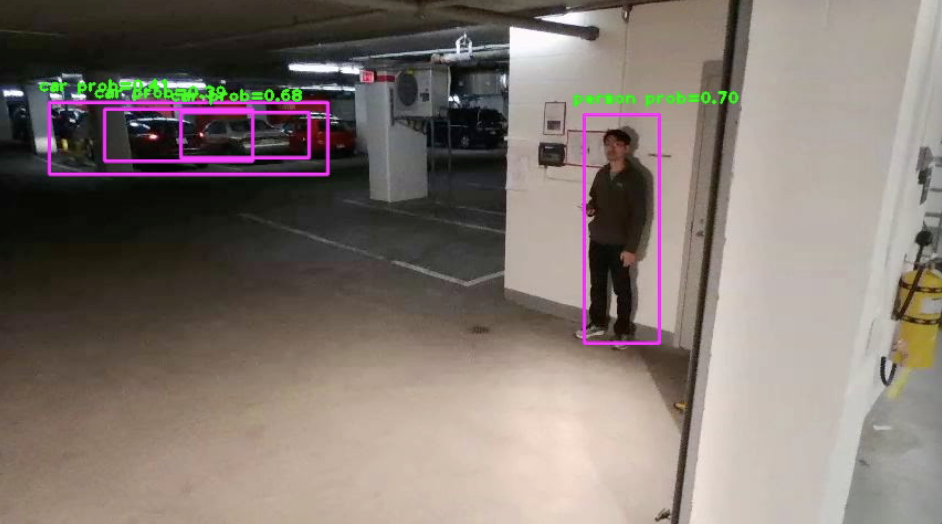
\includegraphics[width=0.35\linewidth]{02-quad-cam}
    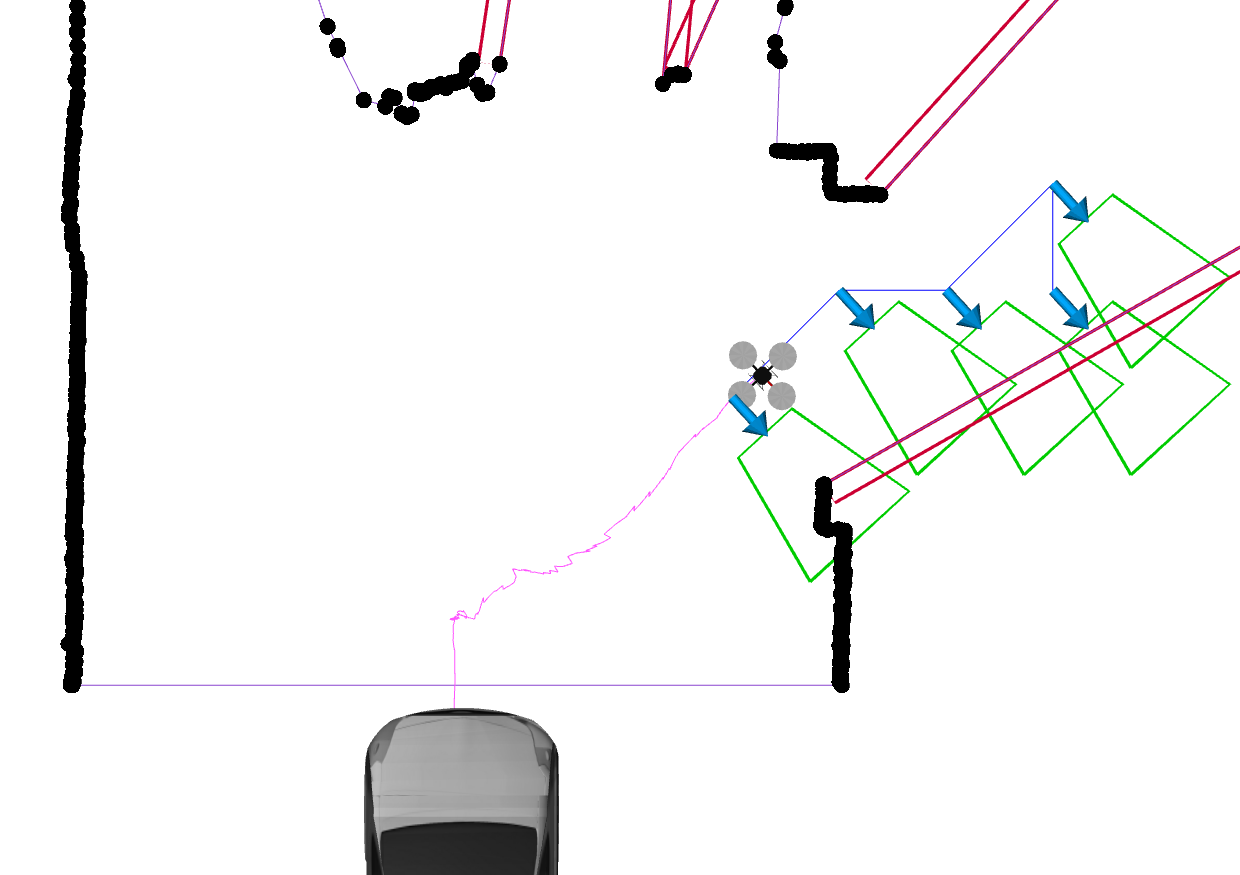
\includegraphics[width=0.28\linewidth]{02-planner-step}

    \caption{}

    \label{fig:experiment}

\end{figure}

\subsubsection{Landing On the Car}

Once the car is ready to park, the quadrotor is able to autonomously land back
on the platform attached to the front bumper.

\begin{figure}[h!]

    \centering

    \centerline{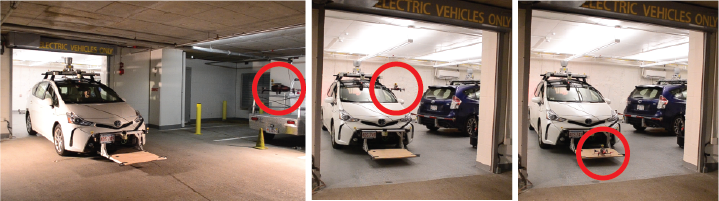
\includegraphics[width=1\linewidth]{landing_sequence}}

    \caption{}

    \label{fig:experiment}

\end{figure}
